%!TEX program = xelatex
%-*- coding: UTF-8 -*-
\documentclass{bjutthesis}
\usepackage{lipsum, zhlipsum}
%\usepackage{layout, showframe}

\ezsetkeys{%
	clc            = {TU311},
	udc            = {004},
	schoolcode     = {10005},
	secretlevel    = {公开},
	studentid      = {S201904283},
	ctitle         = {\bjutthesis~\version\,——北京工业大学硕士学位论文\LaTeX 模板},
	cauthor        = {林钰辉},
	cdiscipline    = {建筑与土木工程},
	cmajor         = {城市水系统健康循环与水环境恢复技术},
	cdegree        = {工学硕士},
	csupervisor    = {张永祥},
	csupervstitle  = {教授},
	ccollege       = {城市建设学部},  
	cdate          = {\the\year 年\the\month 月},
	corganization  = {北京工业大学},
	%% ==== 英文
	etitle         = {\bjutthesis: A~\LaTeX~Template for Doctral Dissertation of Beijing University of Technology},
	edegree        = {Doctor of Engineering},
	emajor         = {Basketball},
	eauthor        = {YAO Ming},
	esupervisor    = {DU Xiuli}
}

\makeatletter
\begin{document}
\begin{sloppypar}
\makecover
\maketitle
\makestate
\makeatother
\frontmatter
\begin{cabstract}
	纳米零价铁(nZVI)越来越多地用于污染土壤和含有氯化溶剂和重金属的地下水的原位修复。但分散在水相中的纳米零价铁颗粒由于磁力作用而具有强烈的聚集趋势,形成远超过微米尺寸的枝状絮体和网状结构,降低了它的有效表面积和反应活性在实验室研究和现场试验中的迁移性和稳定性表现均不理想。因此研究纳米零价铁在多孔介质中的迁移,通过制备改性纳米铁增强其稳定性与分散性,提高其在多孔介质中的迁移距离。并通过填充柱实验,研究硫化型纳米零价铁在多孔介质中的迁移过程以及多孔介质水力特性的变化过程。建立考虑拦截、布朗扩散、重力沉降和多孔介质性质变化影响的非稳态变参数数学模型。通过模型与实验数据的拟合,研究实验过程中各种机理的变化。
	\ckeywords{包覆型硫化型纳米铁;颗粒稳定性;XDLVO;多孔介质;迁移}
\end{cabstract}

\begin{eabstract}
	Nanometer zero-valent iron (nZVI) is increasingly used for in situ remediation of contaminated soils and groundwater containing chlorinated solvents and heavy metals.  However, due to the magnetic force, the zero-valent iron nanoparticles dispersed in the aqueous phase have a strong tendency to aggregate and form dendritic flocs and network structures with a size far larger than micron, which reduce their effective surface area and reactivity. Their mobility and stability are not ideal in laboratory and field tests.  Therefore, the migration of zero-valent iron nanoparticles in porous media was studied, and its stability and dispersion were enhanced by preparing modified iron nanoparticles to improve its migration distance in porous media.  The migration process of sulfurized zero-valent iron nanoparticles in porous media and the change process of hydraulic characteristics of porous media were studied by packed column experiment.  A mathematical model of unsteady variable parameters considering interception, Brownian diffusion, gravity settlement and property change of porous media is established.  By fitting the model with experimental data, the changes of various mechanisms in the experimental process are studied.  
	\ekeywords{Sulfidated nanoscale zero valent iron, Dispersion stability,Extended DLVO, Porous medium, Transport}
\end{eabstract}
\makebitoc

\mainmatter
\bichapter{绪论}{introduction}

\bisection{研究目的及意义}{Purpose and significance of the study}

纳米零价铁(NZVI)因为独特的物理和化学性质,如高界面反应性显示出在处理废水中有机污染物方面具有巨大潜力;极小的粒径使NZVI可以直接注入受污染的含水层中\cite{2}。因此NZVI越来越多地用于污染土壤和含有氯化溶剂和重金属的地下水的原位修复\cite{1,WOS:000704630800008,REN2022127322,LI201916}。然而,研究表明,纳米零价铁在实验室研究和现场试验中的迁移性和稳定性表现均不理想\cite{3}。主要原因在于分散在水相中的纳米零价铁颗粒由于磁力作用而具有强烈的聚集趋势,形成远超过微米尺寸的枝状絮体和网状结构,降低了它的有效表面积和反应活性\cite{4},以及NZVI的高表面活性导致其常在与污染物接触前被氧化,于表面形成铁氧化物外壳,导致NZVI活性降低\cite{HUANG2016168}。同时,砂粒表面在中性条件下带负电,零价铁颗粒易吸附在其表面上\cite{5},使得零价铁在多孔介质中不易扩散。因此研究纳米零价铁在多孔介质中的迁移,增强纳米铁的稳定性与分散性,提高其在介质中的迁移距离,对实现 NZVI 颗粒在可操作条件下成功运送至“反应区域”具有重要意义。

\bisection{纳米零价铁的研究现状}{NZVI}

零价铁(Zero-Valent Iron,ZVI)由于具有很强的还原能力(E0 = -0.44 V)和吸附重金属、金属等一系列重要污染物的能力,在环境修复中得到了广泛的研究\cite{6}。Gould\cite{7}报道了ZVI在环境中的最早应用,他研究了金属铁丝还原六价铬的动力学。使用纳米零价铁(Nano Zero-Valent Iron, NZVI)在地下进行原位脱氯的概念首先由Wang和Zhang\cite{8}提出,他们假设nZVI可以直接注入受污染的地下水中,并有助于污染土壤和地下水的原位修复\cite{1}。Wang和Zhang\cite{8}证明了合成的、不稳定的ZVI颗粒用于还原脱氯的有效性,并指出新制备的ZVI颗粒比商业铁粉的活性高得多。Zhang等\cite{9}还报道了添加少量催化剂(Pd)可使表面积归一化速率常数增加约100倍。然而所有这些开创性的工作都是在水溶液中进行的,并没有解决与土壤修复相关的其他关键问题,如nZVI易钝化、易流失、颗粒易聚集,土壤输送能力差等。随后,技术进入了一个强调颗粒稳定和迁移性的新阶段。

nZVI的稳定化可以通过表面改性和(或)创建分离纳米粒子的网络来实现,如\cref{fig1}所示。nZVI的稳定剂可分为表面活性剂、合成或天然大分子或高分子电解质、粘度调节剂、油乳化剂和微尺度固体载体。 

\begin{figure}[h]
    \centering
    \begin{subfigure}{.4\textwidth}
		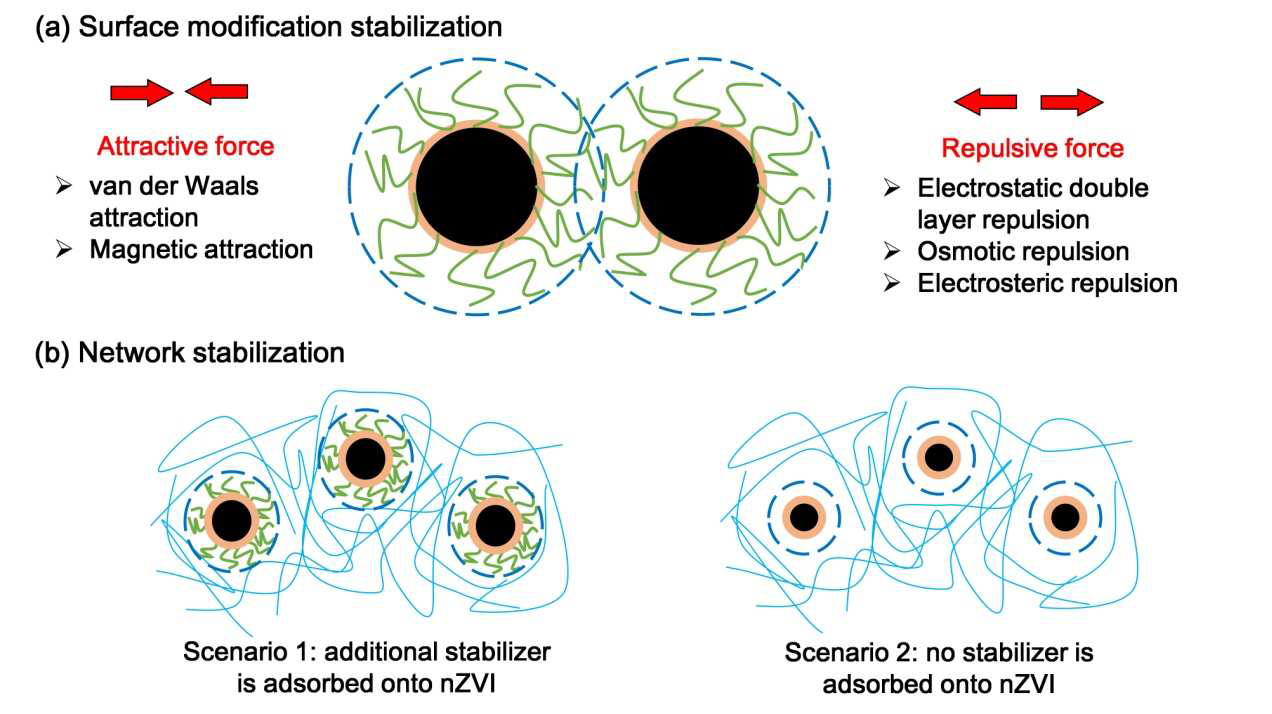
\includegraphics[width=\textwidth]{figs/fig1.png}
	\end{subfigure}
	\begin{subfigure}{.4\textwidth}
		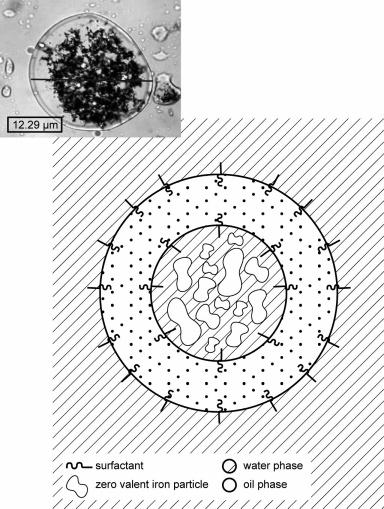
\includegraphics[width=\textwidth]{figs/fig2.png}
	\end{subfigure}
    \bicaption{(a)纳米零价铁稳定化示意图(b)EZVI液滴示意图}{(a)Schematic diagram of stabilized NZVI (b)Schematic diagram of EZVI droplets}\label{fig1}
\end{figure}

硫化纳米零价铁(Sulfidated Nanoscale Zero Valent Iron, S-NZVI)是一种对 NZVI 进行表面钝化的改性方法,在原有的零价铁内核-氧化物外壳结构的基础上,再形成了一层铁硫化物的外壳($\mathrm{FeS_x}$),该$\mathrm{FeS_x}$保护层可以有效的防止内层的NZVI内核被周围环境介质氧化\cite{doi:10.1021/acs.est.8b01735}。此外,$\mathrm{FeS_x}$保护层内存在的离域电子有助于电子传递的进行,因此提高了材料对污染物的还原能力,很好地解决了NZVI易钝化的缺点\cite{doi:10.1021/acs.est.8b01735,doi:10.1021/acs.est.6b03997,15}。Kim等\cite{16}发现,硫化条件下形成的纳米零价铁双相材料(Fe/FeS),比仅与氧化铁(Fe/FeO)结合的nZVI更快地还原三氯乙烯(TCE),并且将Fe/FeS暴露于溶解有$\mathrm{Pd}^{2+}$、$\mathrm{Cu}^{2+}$、$\mathrm{N}^{2+}$、$\mathrm{Co}^{2+}$和$\mathrm{Mn}^{2+}$的溶液中可以进一步提高脱氯反应性。然而,由于纳米颗粒的范德华力和零价铁的磁性作用,S-nZVI颗粒仍然会形成团聚体,这大大减少了它们在受污染的地下水中的传输。因此需要对S-NZVI颗粒进行改性,引入克服范德华力和磁性的斥力,以增强S-NZVI的稳定性,从而增强其在地下水中的迁移能力。

表面活性剂是常用的控制颗粒之间的相互作用的稳定剂之一。张永祥、马晓敏等\cite{10}以聚乙二醇( PEG) 为分散剂,在乙醇-水混合溶剂中合成改性纳米零价铁(NZVI)颗粒,讨论了nZVI去除Cr(VI)的影响因素,并对反应产物进行XPS检测。结果表明,乙醇比例为50\%时制备出的纳米零价铁直径在30~60 nm,对Cr(VI)的去除率最高,为95.30\%。NZVI投加量越大,Cr(VI)初始浓度越小,pH越小,温度越高,均有利于水中Cr(VI)的去除。纳米零价铁将Cr(VI)吸附后将其还原为Cr(III),反应过程主要以还原作用为主。

% 目前已有大量关于包覆型NZVI分散性能的研究,基于DLVO理论测定颗粒的$\zeta$电位计算双电层斥力和范德华力,考虑了包覆层提供的空间作用力分析颗粒的稳定效果\cite{doi:10.1080/09593330.2018.1426637},但是考虑包覆层对颗粒表面电荷的影响的研究较少。对于包覆型NZVI,聚合物吸附固定于颗粒表面形成吸附层,同时溶液中的阴阳离子可以穿透软粒子表面,电荷可以分布在颗粒表面和吸附层内部,因此颗粒的电泳迁移率同时受到颗粒表面电势、Donnan电势及带电聚合物的影响\cite{WOS:000692041500001}。因此软粒子的电泳迁移率对滑移面不敏感,$\zeta$电位失去意义,基于硬粒子假设的Smoluchowski理论并不适用\cite{OHSHIMA20152,Ohshima1995}。

% 本文使用海藻酸钠包覆S-NZVI,防止聚集和沉降,提升在地下水中的迁移能力。阴离子聚电解质的使用与颗粒在地下水的流动性相关,因为在地下水中遇到的大多数矿物和天然有机物表面都带负电\cite{YU2020111245,WOS:000243124600047}。因此,阴离子聚电解质包覆层能够提供来自这些表面的静电斥力,以减少粘附现象。利用动态光散射(DLS)测定颗粒的尺寸,计算团聚速率结合沉降实验,评价颗粒的稳定性。使用Ohshima的软粒子理论计算包覆型S-NZVI的表面电势及包覆层的厚度和软度,结合扩展DLVO理论,解释包覆型S-NZVI的团聚机理,利用Smoluchowski团聚动力学模型预测颗粒平均粒径随时间的变化曲线。最后进行柱实验研究不同注入速度和注入浓度对纳米铁在多孔介质中迁移的影响。将颗粒粒径变化带入迁移计算中,预测不同条件下纳米铁再迁移柱中的最大迁移距离。

与表面活性剂相比,合成聚合物和天然聚合物材料已经被更广泛地研究\cite{ZHOU2014155}。聚电解质通过吸附接枝的方式固定于NZVI颗粒表面,形成聚合物包覆层,层内的大分子为包覆粒子提供静电斥力和空间斥力\cite{2018Impact,doi:10.108007388551.2018.1440525}避免其发生团聚。此外,这些大分子不仅能有效地促进NZVI的稳定,还能被微生物降解,作为微生物群落的能量来源。张永祥、常杉等\cite{11} 利用羧甲基淀粉钠(CMS)对nZVI进行包覆改性,利用空间位阻效应提高其分散悬浮性。研究其对2,4-二氯苯酚(2,4-DCP)的去除效果。结果表明,改性后的nZVI直径大约在80~100 nm,呈链状或分散颗粒分布,主要物质组成为零价铁,具有强还原性。当CMS的比例为80.00\%时,悬浮性最佳;经过CMS包覆改性后,nZVI还保留原有的活性,在不同包覆比例对于2,4-DCP的去除效果的实验中发现,同样CMS比例为80\%时去除效果最好,达到83.69\%,且有明显的脱氯降解过程。

乳化型纳米铁的开发是为了针对地下水中高密度非水相液体(Dense nonaqueous-phase liquids,DNPLs)的去除。通常使用食品级表面活性剂、可生物降解的植物油和水将nZVI包装成油滴,即使用油膜包围nZVI,然后疏水油膜涂层使DNAPL浓缩,nZVI将其降解\cite{12},如\cref{fig1}所示。

负载型纳米铁是将微尺度的固体材料作为载体或是支撑材料来稳定nZVI。张永祥、王友好等\cite{13, 14} 研究新制备复合材料改性沸石负载纳米零价铁/镍去除水中2,4-二氯苯酚效果以及该材料在地下水污染原位修复中的应用情况,开展了2,4-二氯苯酚的批实验和柱实验。批实验结果表明, 25℃时,0.6 g的复合材料对20 mg·L-1的2,4-DCP去除效果达到80\%;柱实验结果表明,材料的双金属颗粒分散性良好,避免了团聚现象的出现。

\bisection{纳米零价铁的注入方式}{Nano zero-valent iron injection method}

nZVI的直接注入技术可概括为以下几种方法:

\begin{itemize}
    \item 通过固定注入点将nZVI泥浆引入处理区\cite{17};
    \item 通过气动或水力压裂在注入点周围形成优先流动路径的裂缝网络,并增强nZVI的分布\cite{18};
    \item 通过压力脉冲技术注入nZVI泥浆;
    \item 将nZVI流体混合物与载气相结合,形成可分散到处理区的气溶胶\cite{19};
    \item 通过重力进料注入\cite{20};
    \item 使用携带nZVI的泡沫表面活性剂注入\cite{21}。
\end{itemize}

nZVI在原位修复中的直接注入技术已经较为成熟,基本目的都是将特定量的nZVI泥浆直接注入到含水层中。He等\cite{22}在压力作用下,注入CMC稳定的Fe/Pd纳米材料,用于阿拉巴马北部含水层中四氯乙烯(PCE)、三氯乙烯(TCE)和多氯联苯(PCBs)污染物的原位治理,沿地下水流向共设置4口试验井,在长达596天的试验时间里,纳米材料有助于非生物降解的早期快速进行,长期来看,以CMC为碳源,以非生物/生物过程中的氢为电子供体,促进了现有的生物降解过程,导致了地下水中氯代有机污染物的持续强化破坏。Su等\cite{23}在美国的Parris岛进行了表面修饰型纳米铁材料的现场测试,并对其进行了两年半的监测,以评估对PCE为主的地下源区氯化挥发性有机污染物的处理效果,分别采用了气动注入和固定点注入两种方式,气动注入时能够传输2.1m,但固定点注入只能移动0.89m。Ariel等\cite{24}在加拿大萨尼亚市的一个氯化溶剂污染场地进行现场试验,采用复合改性方式,制得CMC-S-nZVI悬浮液,并通过重力注入到砂质材料中,上游和下游井中收集的样品表明铁颗粒的径向和垂直分布效果优良,行进距离0.9m-2.7m,在地下水中具有稳定的流动性,并且对场地中的多种氯化类有机污染物有着良好的反应活性。

\bisection{本文主要研究内容}{The main research content of this paper}

\subsection{SA-S-NZVI的颗粒稳定性研究}

制备不同包覆比的SA-S-NZVI并研究不同包覆比的沉降曲线;研究不同pH值S-NZVI的$\zeta$电位、不同离子强度各包覆比SA-S-NZVI的电泳迁移率和粒径变化情况,结合Ohshima的软粒子理论计算SA-S-NZVI的表面电势及包覆层的厚度和软度,结合扩展DLVO理论,解释包覆型S-NZVI的团聚机理,利用Smoluchowski团聚动力学模型预测颗粒平均粒径随时间的变化曲线。

\subsection{SA-S-NZVI在多孔介质的迁移性能研究}

通过柱实验研究SA-S-NZVI悬浮液在多孔介质中的运移过程,堵塞的形成、发展过程;堵塞对多孔介质水力特性造成的影响;纳米零价铁在多孔介质中的分布规律;深入分析造成堵塞的机理。

\subsection{技术路线}


% % \begin{multline}
% % \frac{1}{2}\Delta(f_{ij}f^{ij})=
% % 2\left(\sum_{i<j}\chi_{ij}(\sigma_i-\sigma_j)^2+f^{ij}\nabla_j\nabla_i(\Delta f)+\right .\\
% % \left .\nabla_kf_{ij}\nabla^kf^{ij}+f^{ij}f^k\left[2\nabla_iR_{jk}-\nabla_kR_{ij}\right]\vphantom{\sum_{i<j}}\right)
% % \end{multline}


% % 参见\cref{eq:none}:
% % \begin{align}
% % \label{eq:none}
% % &I(X_3;X_4)-I(X_3;X_4\mid{}X_1)-I(X_3;X_4\mid{}X_2)\nonumber\\
% % =&[I(X_3;X_4)-I(X_3;X_4\mid{}X_1)]-I(X_3;X_4\mid{}\tilde{X}_2)\\
% % =&I(X_1;X_3;X_4)-I(X_3;X_4\mid{}\tilde{X}_2)
% % \end{align}

% % \begin{figure}[!htp]
% % 	\centering
% % 	\resizebox{10cm}{!}{\usetikzlibrary{shapes.geometric, arrows}
\tikzstyle{startstop} = [
rectangle,
rounded corners,
minimum width=2cm,
minimum height=1cm,
text centered,
draw=black
]
\tikzstyle{io} = [
trapezium,
trapezium left angle=75,
trapezium right angle=105,
minimum width=1cm,
minimum height=1cm,
text centered,
draw=black
]
\tikzstyle{process} = [
rectangle,
minimum width=2cm,
minimum height=1cm,
text centered,
draw=black
]
\tikzstyle{decision} = [
diamond,
minimum width=2cm,
minimum height=1cm,
text centered,
draw=black]
\tikzstyle{arrow} = [thick, ->, >=stealth]

\begin{tikzpicture}[node distance=2cm]
    \node (pic) [startstop] {待测图片};
    \node (bg) [io, below of=pic] {读取背景};
    \node (pair) [process, below of=bg] {匹配特征点对};
    \node (threshold) [decision, below of=pair, yshift=-0.5cm] {多于阈值};
    \node (clear) [decision, right of=threshold, xshift=3cm] {清晰?};
    \node (capture) [process, right of=pair, xshift=3cm, yshift=0.5cm] {重采};
    \node (matrix_p) [process, below of=threshold, yshift=-0.8cm] {透视变换矩阵};
    \node (matrix_a) [process, right of=matrix_p, xshift=3cm] {仿射变换矩阵};
    \node (reg) [process, below of=matrix_p] {图像修正};
    \node (return) [startstop, below of=reg] {配准结果};
     
    %连接具体形状
    \draw [arrow](pic) -- (bg);
    \draw [arrow](bg) -- (pair);
    \draw [arrow](pair) -- (threshold);

    \draw [arrow](threshold) -- node[anchor=south] {否} (clear);

    \draw [arrow](clear) -- node[anchor=west] {否} (capture);
    \draw [arrow](capture) |- (pic);
    \draw [arrow](clear) -- node[anchor=west] {是} (matrix_a);
    \draw [arrow](matrix_a) |- (reg);

    \draw [arrow](threshold) -- node[anchor=east] {是} (matrix_p);
    \draw [arrow](matrix_p) -- (reg);
    \draw [arrow](reg) -- (return);
\end{tikzpicture}
}
% % 	\bicaption{绘制流程图效果}{Sample Flow Chart}
% % 	\label{fig:flow_chart}
% % \end{figure}

% % \begin{table}[!hpb]
% % 	\centering
% % 	\bicaption[指向一个表格的表目录索引]
% % 	{一个颇为标准的三线表格\footnotemark[1]}
% % 	{ATableExample}
% % 	\label{tab:firstone}
% % 	\begin{tabular}{@{}llr@{}}\toprule
% % 		\multicolumn{2}{c}{Item}\\\cmidrule(r){1-2}
% % 		Animal&Description&Price(\$)\\\midrule
% % 		Gnat&pergram&13.65\\
% % 		&each&0.01\\
% % 		Gnu&stuffed&92.50\\
% % 		Emu&stuffed&33.33\\
% % 		Armadillo&frozen&8.99\\\bottomrule
% % 	\end{tabular}
% % \end{table}




\bichapter{改性硫化型纳米零价铁的颗粒稳定性研究}{Study on stabilization
of coated sulfur-modified NZVI}

\bisection{实验试剂与仪器}{Chemical reagents and instrument analyses}

\subsection{实验试剂}

本文研究主要用到的实验试剂如\cref{tab1}

\begin{table}[h]
	\centering
	\bicaption{主要实验试剂}{Main experimental reagents}
	\label{tab1}
	\begin{tabular}{@{}cccc@{}}
        \toprule
		试剂名称&分子式&纯度&生产厂家\\
        \midrule
		海藻酸钠&X&AR&天津市福晨化学试剂厂\\
		硫化钠&$\mathrm{Na_2S}$&AR&天津市福晨化学试剂厂\\
		硼氢化钠&$\mathrm{NaBH}$&AR&天津市福晨化学试剂厂\\
		硫酸亚铁&$\mathrm{FeSO_4\cdot7H_2O}$&AR&天津市福晨化学试剂厂\\
		盐酸&$\mathrm{HCl}$&AR&天津市福晨化学试剂厂\\
        氢氧化钠&$\mathrm{NaOH}$&AR&天津市福晨化学试剂厂\\
        盐酸羟胺&$\mathrm{HONH_3Cl}$&AR&天津市福晨化学试剂厂\\
        邻菲啰啉&$\mathrm{C_12H_8N_2H_2O}$&AR&天津市福晨化学试剂厂\\
        硫酸亚铁铵&XX&AR&天津市福晨化学试剂厂\\
        乙酸钠&$\mathrm{CH_3COONa}$&AR&天津市福晨化学试剂厂\\
        石英砂&$\mathrm{SiO_2}$&AR&天津市福晨化学试剂厂\\
        氯化钠&$\mathrm{NaCl}$&AR&天津市福晨化学试剂厂\\
        氮气&$\mathrm{N_2}$&LP&北京海瑞通达气体科技有限公式\\
        \bottomrule
	\end{tabular}
\end{table}

\subsection{主要试验仪器}

试验过程中主要使用到的仪器和设备见\cref{tab2}

\begin{table}[h]
	\centering
	\bicaption{主要实验试剂}{Main experimental reagents}
	\label{tab2}
	\begin{tabular}{@{}ccc@{}}\toprule
		仪器名称&规格型号&生产厂家\\\midrule
		精密定时电动搅拌器&JJ-1&北京市中兴伟业仪器有限公司\\
        超声波细胞粉碎机&BILON-650Y&上海比朗仪器制造有限公司\\
		冷冻干燥机&FD-1A-50&上海比朗仪器制造有限公司\\
		流量型蠕动泵&BT100-1L&保定兰格恒流泵有限公司\\
		紫外可见分光光度计&2082S UV/VIS&上海尤尼柯仪器有限公司\\
		电子天平&JA2003&上海恒平科学仪器有限公司\\
        Zeta电位及粒度分析仪&90Plus Zeta&美国布鲁克海文仪器公司\\
        真空干燥箱&DZ-2AII&天津市泰斯特仪器有限公司\\\bottomrule
	\end{tabular}
\end{table}

\bisection{材料制备和研究方法}{Materials and methods}

\subsection{海藻酸钠改性硫化型纳米铁的制备}\label{material}

用于制备SA-S-NZVI的海藻酸钠和硫化钠购自天津市福晨化学试剂厂。超纯水(SIM-T30UV,北京飞翔赛思科技有限公司)在反应前通过氮气(北京顺驰东环干冰经营中心)进行脱氧。实验的所有试剂均为分析纯,所有溶液和稀释液均在超纯水中制备。

采用表面腐蚀法制备S-nZVI,$\mathrm{S^{2-}}$水解产生$\mathrm{HS^-}$和$\mathrm{H_2S}$对nZVI具有腐蚀作用,生成的$\mathrm{Fe^{2+}}$与$\mathrm S^{2-}$结合,在nZVI表面生成FeS\cite{ ISI:000382805800072}。使用液相还原法制备NZVI\cite{2020The,LIU2019124193},将2.48 g$\mathrm{FeSO_4\cdot 7H_2O}$ 溶解于350 ml超纯水中。取0.68 g$\mathrm{NaBH_4}$溶于150 ml超纯水后逐滴加入到上述溶液中。同时用电动搅拌机(JJ-1,北京市中兴伟业仪器有限公司)以600 $\mathrm{r\cdot min^{-1}}$的转速搅拌,反应完成后继续搅拌15 min,反应式如\cref{eq1}。将混合液过滤,收集的固体颗粒用去离子水冲洗2次,无水乙醇冲洗1次,将其干燥后密封置于冰箱中保存。配置1 g/L的NZVI悬浊液,超声10 min,向其中加入0.32 g $\mathrm{{Na}_2S}$,使用电动搅拌机搅拌2 h,获得S/Fe比(摩尔比)为0.15的S-nZVI。其反应式如\cref{e16}所示\cite{ ISI:000355774400014}。

\begin{equation}\label{eq1}
    \mathrm{{Fe}^{2+}+2{BH}_4^-+4H_2O}\rightarrow \mathrm{2{Fe}^0\left(s\right)+{B\left(OH\right)}_4^-+4H^+}\mathrm{+2H_2\left(g\right)}
\end{equation}
\begin{equation}
    \mathrm{{Na}_2S+H_2O\rightarrow2{Na}^++{HS}^-+{OH}^-}
\end{equation}
\begin{equation}
    \mathrm{{Fe}^{2+}+2{HS}^-\rightarrow FeS(s)+H_2S}
\end{equation}
\begin{equation}\label{e16}
    \mathrm{S^{2-}+{Fe}^{2+}\rightarrow FeS(s)}
\end{equation}

将0.5 g的S-NZVI颗粒分别分散在不同浓度的海藻酸钠的水溶液中(0.0、0.1、0.2、0.3 wt\%),超声处理30 min。然后27500 rpm转速离心80 min,倒去上清液,用超纯水清洗数次后干燥备用。样品依次记为S-NZVI,0.1\%SA-S-NZVI,0.2\%SA-S-NZVI和0.3\%SA-S-NZVI。

\subsection{电泳迁移率的测定}

将S-NZVI悬浮于0.1 mM的NaCl溶液中,使用NaOH或HCl调整溶液pH,使用超声细胞粉碎机中超声30 min。使用Zeta电位及粒度分析仪(90Plus Zeta, Brookhaven Instruments Corporation)测定不同pH在3到10范围内S-NZVI的电泳迁移率($u_e$)。S-NZVI的$\zeta$电位由Smoluchowski方程计算:$\zeta=\eta u_\mathrm{e}/\varepsilon$。其中$\eta$为水粘度,$\varepsilon$为水的介电常数。将\cref{material}制备完成的4种样品分别悬浮于不同离子强度的NaCl溶液中(5.0,10.0,20.0,40.0,60.0,80.0 mM),调节溶液pH为8,测定样品的电泳迁移率。

\subsection{沉降速率的测定}

使用0.1 mM NaCl溶液将\cref{material}制备完成的4种样品配置成1.0 g/L的悬浮液,调整溶液pH=8放入石英比色皿,使用紫外分光光度计(2082S UV/VIS,Unico Instrument Corporation)在508 nm波长下测定不同时刻对铁的吸光度,扫描时间4000 s,扫描间隔30 s。

\subsection{颗粒尺寸的测定}

利用Zeta电位及粒度分析仪(90Plus Zeta, Brookhaven Instruments Corporation)的动态光散射(DLS)模块测定SA-S-NZVI纳米颗粒的颗粒尺寸($a_\mathrm{h}$)。将上述样品配置成0.015 g/L的悬浮液,使用NaOH或HCl调整溶液pH=8,于氮气气氛超声30 min后立即测量。散射光由光电探测器以$90^\circ$散射角检测,每次检测60 s。根据瑞利近似,散射光强度与粒径的六次方正相关,因此强度分布对粒径特别敏感,不适用与宽分布样品(图 S1)。为了有效确定团聚颗粒的粒径分布,对比了DLS的强度平均(by intensity)数据和数量平均(by number)数据。本文选择使用水力粒径的数量平均值以表征颗粒的尺寸分布。

\subsection{附着效率计算}

通过计算初始团聚速率常数$k$和附着效率$(\alpha)$来表征SA-nZVI的团聚动力学。团聚行为刚开始时,水力半径$a_\mathrm{h}$与时间$t$呈线性关系。因此,初始团聚速率常数($k$)可以通过对$a_\mathrm{h}(t)$随t的变化量进行线性最小二乘回归分析得到。该回归分析通常在从$t = 0$到$a_\mathrm{h}(t)$的值达到$1.25a(0)$的时间范围内进行\cite{ChenElimelech-762}。由\cref{1-20}计算不同离子强度下颗粒的初始团聚速率\cite{ChenMylon-760}:

\begin{equation}\label{1-20}
    k\propto\frac{1}{N_0}\left(\frac{\mathrm{d}a_\mathrm{h}(t)}{\mathrm{d}t}\right)_{t\rightarrow0}
\end{equation}

其中,$N_0$为纳米颗粒悬浊液的初始浓度。附着效率$\alpha_{\mathrm {pp}}$反映了颗粒之间发生有效碰撞的几率。它被定义为反应受限团聚(并非所有的碰撞都是有效的,团聚的发生需要颗粒的能量超过反应势垒,因此碰撞效率($\alpha_\mathrm{pp}<1$)与扩散受限团聚(聚集的发生由布朗运动引起,只要颗粒发生接触,就会形成更大的团簇,即碰撞效率($\alpha_\mathrm{pp}=1$)。导出的团聚速率之比\cite{doi:10.1021/la062072v}:

\begin{equation}\label{alpha_ppexp}
  \alpha_{\mathrm{pp}}=\frac{k}{k_{\mathrm{fast}}}=\frac{\frac{1}{N_0}\left(\frac{\mathrm{d}a_\mathrm{h}(t)}{\mathrm{d}t}\right)_{t\rightarrow0}}{\frac{1}{N_{0,\mathrm{fast}}}\left(\frac{\mathrm{d}a_\mathrm{h}(t)}{\mathrm{d}t}\right)_{t\rightarrow0,\mathrm{fast}}}
\end{equation}

其中,下标“fast”指扩散受限团聚。$k_{\mathrm{fast}}$取扩散限制团聚阶段下$k$的平均值。

\subsection{聚电解层厚度计算}

由于溶液中的阴阳离子和电荷可以透过包覆型S-NZVI表面,分布在吸附层内部,因此测量电泳迁移率结合Ohshima的软粒子理论来确定聚电解质吸附层的特性。Ohshima认为,软粒子周围的电势由吸附层内厚度为$d$的Donnan电势($\psi_\mathrm{DON}$)和吸附层与溶液边界的表面电势($\psi_\mathrm{0}$)组成\cite{2006315,OHSHIMA20152,Ohshima1995}(\cref{donnan})。结合Navier-Stokes方程计算吸附层的摩擦力,软粒子的电泳迁移率的表达式为\cite{Oshima1992}:

\begin{equation}\label{psidon}
    \psi _\mathrm{DON}=\frac{k_BT}{ze_0}\ln[\frac{ZN}{2zn}+\{(\frac{ZN}{2zn})^2+1\}^{1/2}]
\end{equation}
\begin{equation}\label{psi0}
    \psi_0=\psi_\mathrm{DON}-\frac{k_BT}{ze_0}\tanh\frac{ze_0\psi_\mathrm{DON}}{2k_BT}+\frac{4k_BT}{ze_0}\cdot e^{-\kappa_md}\cdot\tanh\frac{ze_0\zeta }{4k_BT}
\end{equation}
\begin{equation}
    \kappa=\sqrt{\frac{2nz^2e_0^2}{\varepsilon k_B T}}
\end{equation}
\begin{equation}
    \kappa_\mathrm{m}=\kappa\sqrt{\cosh(\frac{ze_0\psi_\mathrm{DON}}{k_BT})}
\end{equation}
\begin{align}\label{ue}
    u_\mathrm{e}=&\frac{\varepsilon}{\eta }\cdot\frac{\psi _0/\kappa _m+\psi _\mathrm{DON}/\lambda }{1/\kappa _m+1/\lambda }\cdot\frac{2}{3}\cdot[1+\frac{1}{2(1+d/a)^3}]\\ &+\frac{Ze_0N}{\eta \lambda ^2}+\frac{8\varepsilon k_BT}{\eta \lambda ze_0}\cdot\tanh \frac{ze_0\zeta}{4k_BT}\cdot\frac{e^{-\lambda d}/\lambda -e^{-\kappa _md}/\kappa _m}{1/\lambda ^2-1/\kappa _m^2}\nonumber
\end{align}

其中,$Z$为聚电解质电离基团的价态;$N(\mathrm{m^{-3}})$为包覆层中聚电解质的浓度;$z$为水相中电解质的价态(本文中使用NaCl,z取1);$n$为电解质的浓度;$e_0$为电子电荷;$k_\mathrm{B}$为玻尔兹曼常数;$\kappa_m$为有效徳拜常数;$a$、$d$分别为颗粒粒径和包覆层厚度;$\zeta$为裸S-NZVI的$\zeta$电位;$1/\lambda$为参数,其大小代表聚电解质层的软度,当$1/\lambda\rightarrow 0$时,包覆层为刚性,此时\cref{ue}等价于Smoluchowski方程。测定不同离子强度下裸S-NZVI和包覆型S-NZVI的电泳迁移率用于拟合\cref{psidon,psi0,ue}得到$N$、$\lambda$和$d$。

\begin{figure}
    \centering
    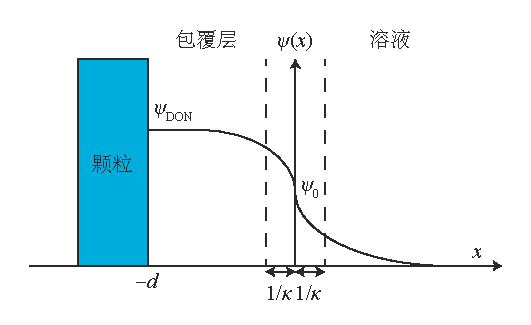
\includegraphics[width=8cm]{figs/Donnan-potential.pdf}
    \bicaption{软粒子表面的电势示意图}{Schematic diagram of the electric potential on the surface of a soft particle}\label{donnan}
\end{figure}

\subsection{碰撞频率的计算}

碰撞频率函数反映的是颗粒在分散体系中单位时间碰撞的次数。水环境中,粒子碰撞的机制主要为三种:布朗运动、流体剪切和差速沉降\cite{ThomasJudd-749}。采用Coalesced Fractal Sphere(CFS)模型\cite{LeeBonner-748}:(1)所有的絮凝体由单一类型的初级颗粒组成,这些初级颗粒是致密的球体。(2)所有絮凝体都具有固定的分形维数,且不受絮凝体粒径的影响。(3) 当两个絮凝体碰撞并结合时,新形成的絮凝体具有与碰撞前絮凝体相同的分形维数,新絮凝体的固体体积是碰撞前絮凝体的固体体积之和。布朗运动、流体剪切和差速沉降三种碰撞频率函数$\beta_{BR}$、$\beta_{SH}$、$\beta_{DS}$按下式计算\cite{LeeBonner-748}:
\begin{equation}\label{beta_br}
    \beta_{BR}(v_i,v_j)=\frac{2kT}{3\mu}(v_i^{1/D_F}+v_j^{1/D_F})(v_i^{-1/D_F}+v_j^{-1/D_F})
\end{equation}
\begin{equation}\label{beta_sh}
    \beta_{SH}(v_i,v_j)=\frac{G}{\pi}v_0^{1-3/D_F}{(v_i^{1/D_F}+v_j^{1/D_F})}^3
\end{equation}
当$D_F\in[2,3]$时
\begin{align}\label{beta_ds}
    \beta_{DS}(v_i,v_j)=&\frac{g}{12\mu}{(\frac{\pi}{6})}^{-1/3}[(\rho_0-\rho_w)/\rho_w]v_0^{1/3-1/D_F}\\ & \times(v_i^{1/D_F}+v_j^{1/D_F})^2\left|v_i^{(D_F-1)/D_F}-v_j^{(D_F-1)/D_F}\right| \nonumber
\end{align}
当$D_F\in[0,2]$时
\begin{align}
    \beta_{DS}(v_i,v_j)=&\frac{g}{12\mu}{(\frac{\pi}{6})}^{-1/3}[(\rho_0-\rho_w)/\rho_w]v_0^{4/3-3/D_F}\\ &\times(v_i^{1/D_F}+v_j^{1/D_F})^2\left|v_i^{1/D_F}-v_j^{1/D_F}\right| \nonumber
\end{align}
式中$v_0$为颗粒体积,$v_i$和$v_j$分别为不同絮凝体的固体体积,$\rho_0$为单体密度,$\rho_w$为水密度,$D_F$为分形维数。

\subsection{团聚动力学模型}

Von Smoluchowski在1917年提出了团聚动力学方程\cite{Smoluchowski-752},在胶体化学的范畴内,在忽略重力、无絮体分裂、无介质流动、絮体沿直线相互碰撞等假设的简化条件下,在数学上反映团聚过程中不同粒径颗粒的团聚过程\cite{Smoluchowski-752}:

\begin{equation}\label{smoluchowski}
    \frac{\mathrm{d}n_k}{\mathrm{d}t}=\frac{1}{2}\alpha_\mathrm{pp}\sum_{i+j=k}{\beta(i,j)n_in_j}-\alpha_\mathrm{pp} n_k\sum_{i=1}^{z}{\beta(i,k)n_i}
\end{equation}

式中,右下角标代表形成对应阶数聚集体消耗的初级颗粒数量,对应$n_i$、$n_j$、$n_k$分别为对应阶数的聚集体浓度($\mathrm{m^{-3}}$);$z$为其中构成最大絮凝体消耗的初级颗粒数量($i$,$j$,$k\leq z$);$\alpha_\mathrm{pp}$表示碰撞效率由\cref{alpha_ppexp}计算;$\beta$是与两个碰撞颗粒体积相关的函数由\cref{beta_br,beta_sh,beta_ds}计算。方程右侧的第一项表示$i$阶团聚体和$j$阶团聚体碰撞形成阶数为$k$的团聚体的速率,第二项表示$k$阶团聚体与其他团聚体碰撞后损失的速率。第一项前的1/2确保了在求和过程中,相同的碰撞不会被计算两次。方程定义了$k$阶团聚体浓度的变化速率。

\bisection{结果与讨论}{Results and discussion}

\subsection{pH对不同包覆比的S-NZVI稳定性的影响}

如\cref{fig3}所示,未包覆的S-NZVI在酸性条件下时$\zeta$电位为正,碱性条件下为负,等电点在pH=7.0附近,此时颗粒表面静电力变小,排斥力减弱。由于通常地下水的pH范围在6.5到8.5之间\cite{dixiashuibiaozhun},因此该环境下未包覆的S-NZVI胶体团聚速率快,更易脱稳沉降,与相关研究结果相符。为模拟地下水环境,调节pH=8,因此本研究中的硫化纳米铁表面带负电。

\begin{figure}[h]
    \centering
    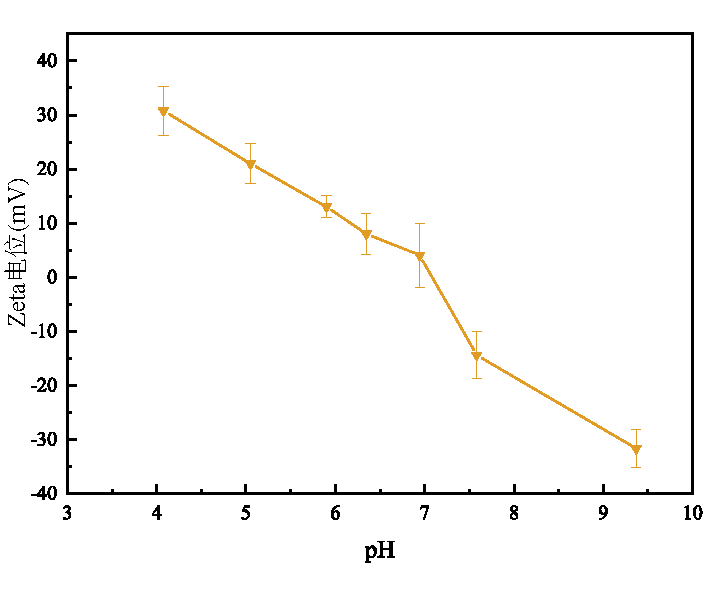
\includegraphics[width=8cm]{figs/fig3.pdf}
    \bicaption{不同pH裸S-NZVI的$\zeta$电位}{Zeta potential of bare S-NZVI as a function of pH}\label{fig3}
\end{figure}

\subsection{不同包覆比下S-NZVI的稳定性}

纳米颗粒在水中同时受到扩散和重力沉降作用,如果纳米粒子的扩散克服了沉降作用,那么纳米粒子可以保持很长时间的稳定。其中重力作用与粒子半径的平方成正比,扩散作用与粒子尺寸成反比,当纳米粒子聚集成微米大小的团簇时,由于扩散作用小于沉降作用,团聚体会沉降到容器的底部。所以沉降速率是表征S-NZVI胶体稳定性的良好指标。

\begin{figure}[h]
    \centering
    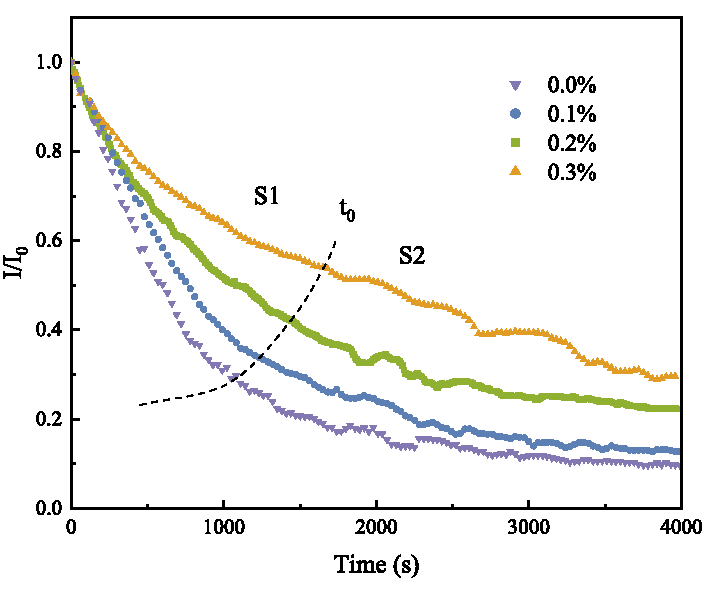
\includegraphics[width=8cm]{figs/fig1.pdf}
    \bicaption{不同包覆比和裸S-NZVI的沉降曲线}{Sedimentation curves of bare and modified S-NZVI}\label{fig01}
\end{figure}

如\cref{fig01}所示,未包覆的S-NZVI的沉降可分为两个阶段:在S1阶段,样品中存在大量超过临界尺寸的颗粒,因此快速沉降。在$t_0$时刻,多数大颗粒沉降完成,沉降速率降低,样品进入S2缓慢沉降阶段,逐渐趋于稳定。

海藻酸钠包覆S-NZVI的沉降模式与未包覆材料相同,均由S1、S2两个阶段组成,但由于聚电解质层的存在,包覆硫化钠米铁的沉降速率与海藻酸钠浓度负相关。海藻酸钠浓度越大,S1阶段的沉降速率越小,S2阶段保持悬浮的颗粒数量越多,体系的稳定性越好。

\subsection{离子强度对SA-S-NZVI稳定性的影响}

金属氧化物纳米颗粒在水溶液中的稳定性在很大程度上取决于离子强度。为了研究离子强度对SA-S-NZVI在溶液中的稳定性(pH=$8\pm 0.1$),制备不同包覆比(0、0.1、0.2、0.3wt\%)的SA-S-NZVI,采用NaCl调节离子强度(0.00$\sim$100 mM NaCl)。颗粒之间的附着效率由\cref{alpha_ppexp}计算,其中$k_{\mathrm{fast}}$取扩散限制团聚阶段下$k$的平均值。

\begin{figure}[h]
    \centering
    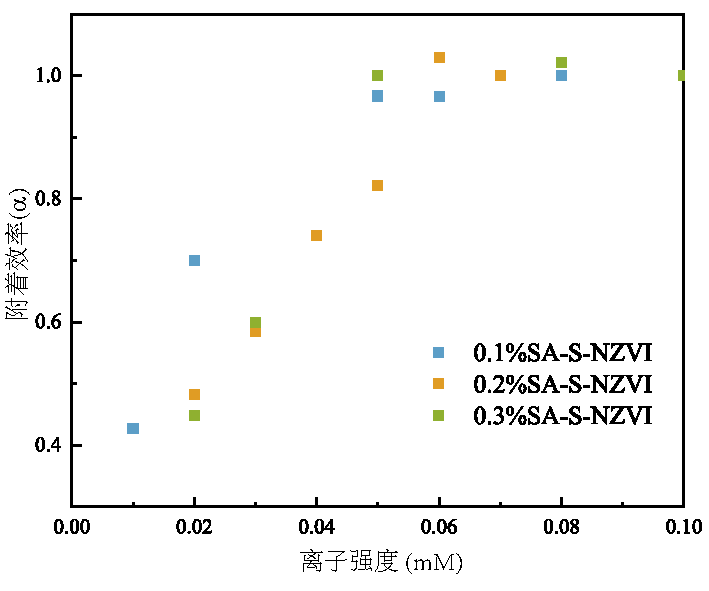
\includegraphics[width=8cm]{figs/Graph1.pdf}
    \bicaption{不同离子强度下包覆型S-NZVI的附着效率}{Influence of iron strength on aggreation behaviors of modified S-NZVI}\label{fig4}
\end{figure}

实验结果如\cref{fig4}所示,不同包覆比的SA-S-NZVI与裸S-NZVI随着离子强度的增加,在低浓度NaCl下,NaCl浓度的增加将提高电荷屏蔽的程度,从而提高团聚速率,这反映在附着效率的提高上。该过程中,附着效率与NaCl的投加量正相关,这种团聚过程称为反应限制团聚$(\alpha<1)$。在高NaCl浓度下,SA-NZVI的电荷被完全屏蔽,势垒消失,该过程中颗粒发生扩散限制团聚$(\alpha=1)$,团聚速率达到最大值,且与NaCl投加量无关。NaCl对不同包覆比S-NZVI的临界浓度均在0.05\textasciitilde0.06 mM附近。

\subsection{聚电解质包覆层的特性}

颗粒间空间斥力的大小和作用范围与表面吸附的聚合物浓度和包覆层厚度有关。不同包覆比的S-NZVI的电泳迁移率随离子强度的变化如\cref{fig5}所示,其中曲线由测量的平均电泳迁移率\cref{psidon,psi0,ue}拟合得到,各参数见\cref{tb1}。

由于包覆层的存在,SA-S-NZVI周围的扩散层被压缩,其电泳迁移率随离子强度的变化较未包覆S-NZVI小。随着离子强度不断提高,未包覆S-NZVI的电泳迁移率逐渐趋于零,而不同包覆比的SA-S-NZVI(0.1\%wt,0.2\%wt,0.3\%wt)受包覆层特性影响分别趋于-2.8,-2.2和-2.3 $\mathrm{\mu m\, s^{-1}\, cm\,V^{-1}} $。

由于软粒子对滑移面位置不敏感\cite{1992Electrophoretic},Smoluchoski公式以硬粒子为基础并不适用于包覆型S-NZVI。根据Ohshima的软粒子理论计算的包覆型S-NZVI的表面电荷$\psi_0$远小于由Smoluchoski公式计算的$\zeta$电位。因此,软粒子并不适用于传统DLVO理论的双电层公式计算静电斥力。

\begin{figure}[h]
    \centering
    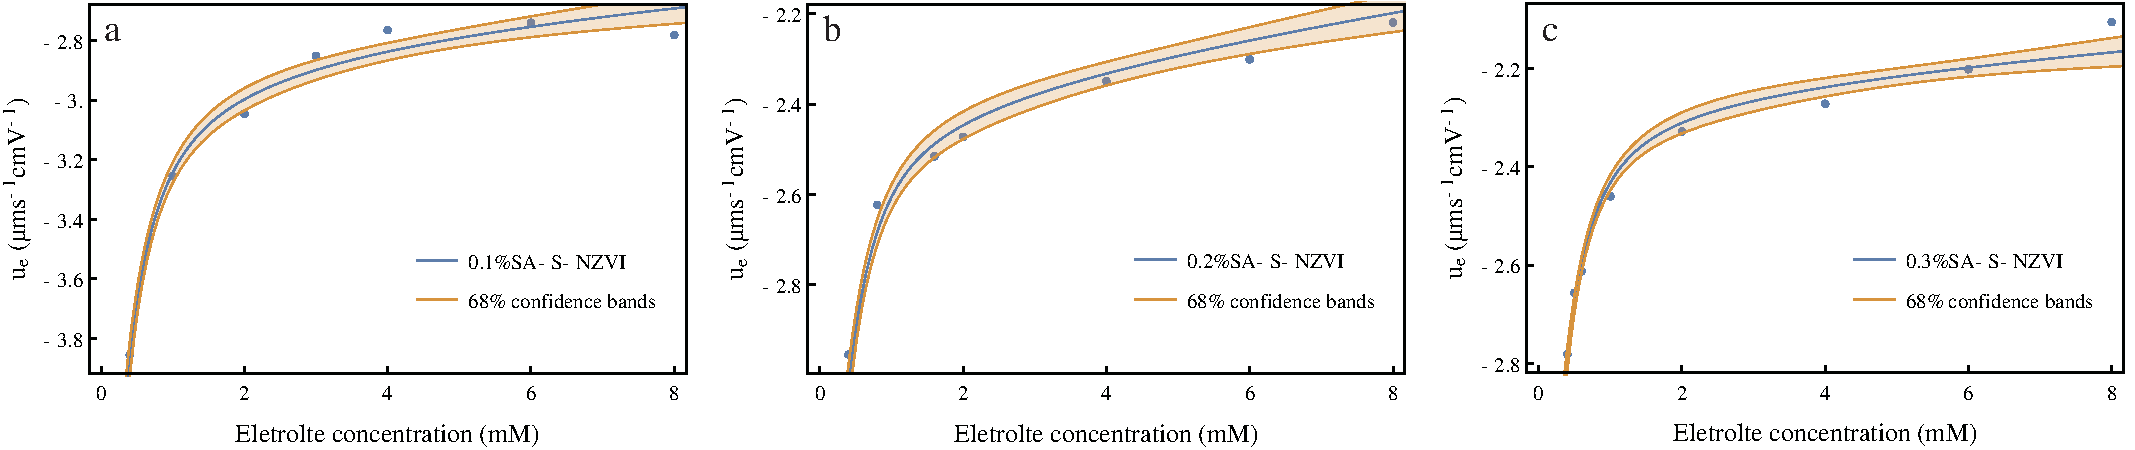
\includegraphics[width=8cm]{figs/fig5.pdf}
    \bicaption{不同NaCl浓度下包覆型S-NZVI的电泳迁移率}{Electiophoretic mobility of the sodium alginate coated S-NZVI as a function of NaCl (mM)}
    \label{fig5}
\end{figure}

\begin{table}
    \centering
    \bicaption{利用Ohshima软粒子理论计算pH值为8.0$\pm $0.1时吸附聚电解质层的特性  }{Characteristics of the adsorbed polyelectrolyte layers at pH 8.0$\pm $0.1 as estimated by Ohshima’s soft particle analysis}\label{tb1}
    \begin{tabular}{@{}ccccc@{}}
        \toprule
         样品类型 & $ZN$/$\mathrm{N_A}$& $d$ & $1/\lambda$ &$\phi_p$\\
           &$(\mathrm{mol/m^3})$&(nm)&(nm)& $(10^{-3})$ \\
        \midrule
        0.1\%SA & 3.28$\pm$1.08 & 7.97$\pm$4.11 & 6.63$\pm$0.58 & 113\\
        0.2\%SA & 1.47$\pm$1.25 & 10.94$\pm$4.68 & 8.51$\pm$1.06 & 80\\
        0.3\%SA & 1.50$\pm$1.39 & 16.62$\pm$4.58 & 9.57$\pm$1.97 & 54\\
        \bottomrule
    \end{tabular}
\end{table}


包覆层中聚电解质的体积分数是影响颗粒稳定性的重要因素。根据计算的颗粒平均包覆层厚度和吸附浓度估算吸附到NZVI表面聚电解质的体积分数:

\begin{align}
    \phi_p=& \frac{\Gamma\cdot 4\pi a^2}{\rho_p\cdot \frac{4}{3}\pi [(d+a)^3-a^3]}  \\
    =&\frac{3\cdot\Gamma a^2}{\rho_p[(d+a)^3-a^3]} \nonumber
\end{align}

其中,$\rho_p$是聚电解质密度;$d$为包覆层厚度;$a$为颗粒粒径;$\Gamma$为S-NZVI表面聚电解质的吸附浓度,制备样品吸附后通过差量法利用总有机碳分析仪测量TOC计算。


\subsection{基于DLVO理论的颗粒相互作用能计算}

未包覆型S-NZVI颗粒在溶液中的稳定性可以用DLVO理论解释\cite{gregory1981approximate,bian2011aggregation}。根据经典DLVO理论,颗粒之间主要吸引能来自范德华力$V_\mathrm{vdW}$,排斥能主要取决于静电双电层的相互作用$V_\mathrm{el}$。求形颗粒之间范德华力的势能大小为\cite{huynh2011aggregation}:

\begin{equation}
    V_{\mathrm {vdW}}=-\frac{A}{6}\{\frac{2a^2}{s(4a+s)}+\frac{2a^2}{(2a+s)^2}+\ln[\frac{s(4a+s)}{(2a+s)^2}]\}
\end{equation}
其中,$A$为Hamaker常数,取$10^{-19}$;$s$为颗粒表面间距;$a$为颗粒半径。在电解质溶液中,当两个带电颗粒相互接近的时候,它们的扩散双电层彼此交迭,并且如果颗粒带电情况相似,它们在接近过程中都将受到排斥作用。根据颗粒大小和双电层厚度的不同,双电层作用$V_{\mathrm{el}}$的计算式如下\cite{bian2011aggregation,noh2010fluorescence,OHSHIMA199545}:
\begin{equation}
    V_{\mathrm{el}}=\left\{
        \begin{array}{lcl}
            4\pi \varepsilon \psi^2\cdot\frac{a_1a_2}{a_1+a_2}\cdot\ln[1+{\mathrm {exp}}(-\kappa s)]& &{\kappa a \geqslant  5}\\
            4\pi \varepsilon Y_1Y_2a_1a_2\cdot(\frac{kT}{e})^2\cdot\frac{{\mathrm {exp}}(-\kappa s)}{a_1+a_2+s}& &{\kappa a < 5}
        \end{array}\right.
\end{equation}

\begin{equation}
    \mathrm{Y_1}=\frac{8\, \tanh[e\psi /(4kT)]}{1+[1-\frac{2\kappa a_i+1}{(\kappa a_i +1)^2} \, \tanh^2[e\psi/(4kT)]] ^{1/2}} 
\end{equation}
\begin{equation}
    \kappa =\sqrt{\frac{1000 e^2 N_A I z_i^2}{\varepsilon k T}}
\end{equation}
其中,$\varepsilon$为水的介电常数,$\psi$为表面电势,未包覆型S-NZVI用$\zeta$电位$(\mathrm V)$替代\cite{wu2013aggregation,bhardwaj2010self,feriancikova2012deposition},SA-S-NZVI的表面电势由软粒子理论计算得到(\cref{tb1})。$k$为是玻尔兹曼常数$(\mathrm {J/K})$,$T$是绝对温度$\mathrm {(K)}$,$\kappa$为徳拜长度的倒数$(\mathrm m^{-1})$,$I$为离子强度$(\mathrm M)$,$e$为单电子的电荷量$\mathrm {(C)}$,$N_\mathrm{A}$为阿伏伽德罗常数$(\mathrm {mol^{-1}})$,由于体系中只有NZVI颗粒,因此$a_1=a_2$,$\mathrm{Y_1=Y_2}$。

由于S-NZVI为纳米零价铁核,表面硫化铁的核壳结构,测量S-NZVI的磁滞回线如\cref{fig6}所示,其饱和磁化强度为1410.62 kA/m,矫顽力大小为20.49 A/m,剩余磁化强度为120.08 kA/mM。因此S-NZVI在水相中的稳定性受到其固有磁矩之间相互作用的影响,即使没有外部磁场干扰,也会因NZVI自身磁矩而相互吸引\cite{butter2003direct}。考虑S-NZVI的磁性对其团聚行为的影响:

\begin{equation}
    V_\mathrm{M}=\frac{-8\pi \mu _0M^2a^3}{9(s/a+2)^3}
    \label{VM}
\end{equation}

其中,$\mu_0$为真空中磁导率$(4\pi\cdot10^{-7}H/m )$;$M$为磁化强度$(\mathrm{A\cdot m^{-1}})$。

\begin{figure}
    \centering
    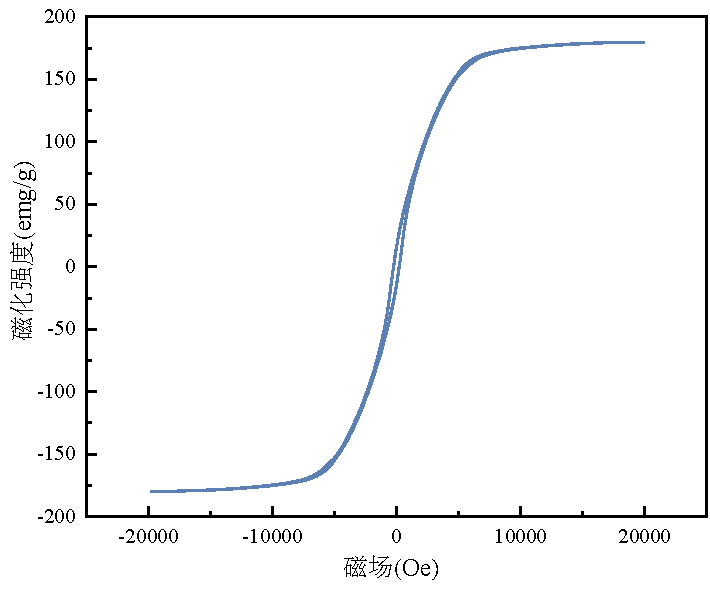
\includegraphics[width=8cm]{figs/fig6.pdf}
    \bicaption{S-NZVI在298.0 K条件下的磁滞回线}{Hysteresis cycle of the magnetization of S-NZVI, at 298.0 K.}
    \label{fig6}
\end{figure}

假设平均粒子半径为50 nm,未包覆型S-NZVI的相互作用如\cref{fig7}所示,其中$V_\mathrm{T}$为相互作用势的总和。此时相互作用力以磁力为主,不存在阻止颗粒聚集的能量势垒,颗粒快速团聚,与观察到的实验现象吻合。

\begin{figure}[h]
    \centering
    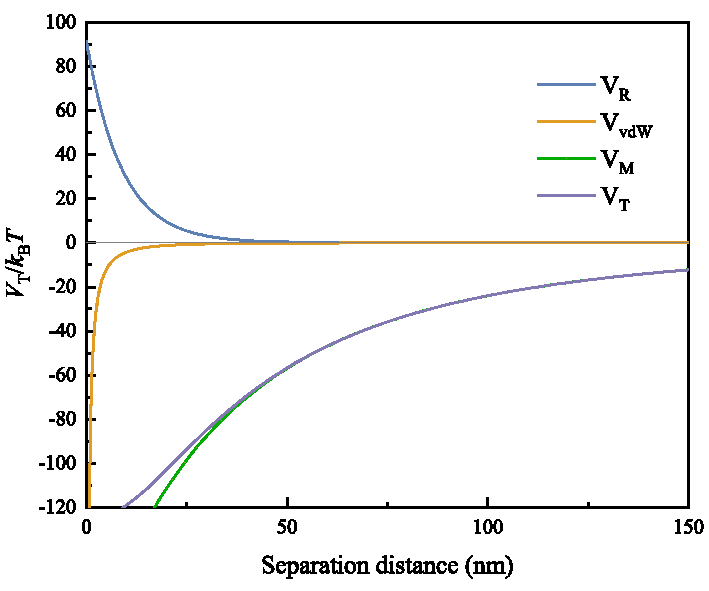
\includegraphics[width=8cm]{figs/fig7.pdf}
    \bicaption{S-NZVI的颗粒间XDLVO相互作用曲线}{Calculated XDLVO interaction energy for bare S-NZVI}
    \label{fig7}
\end{figure}

\begin{figure}[htbp]
    \centering
    \begin{subfigure}{8cm}
		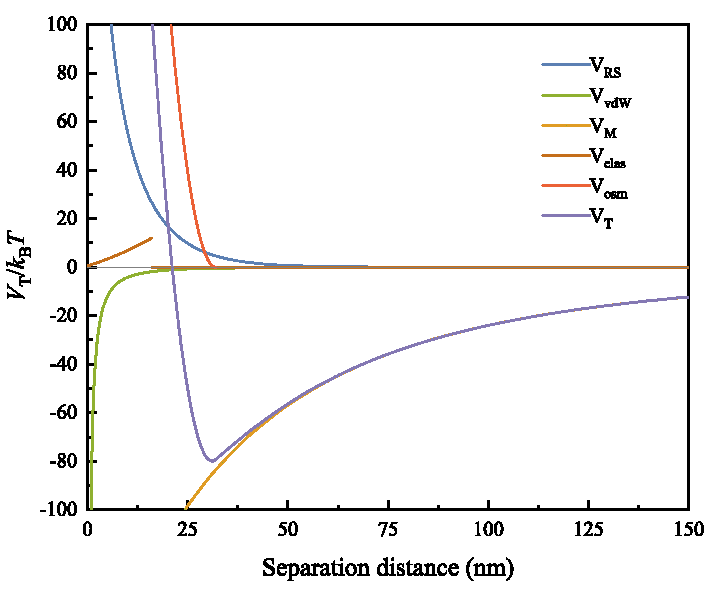
\includegraphics[width=8cm]{figs/fig8.pdf}
        \caption{0.1\%SA-S-NZVI颗粒间相互作用曲线}
        \label{fig8}
	\end{subfigure}

	\begin{subfigure}{8cm}
		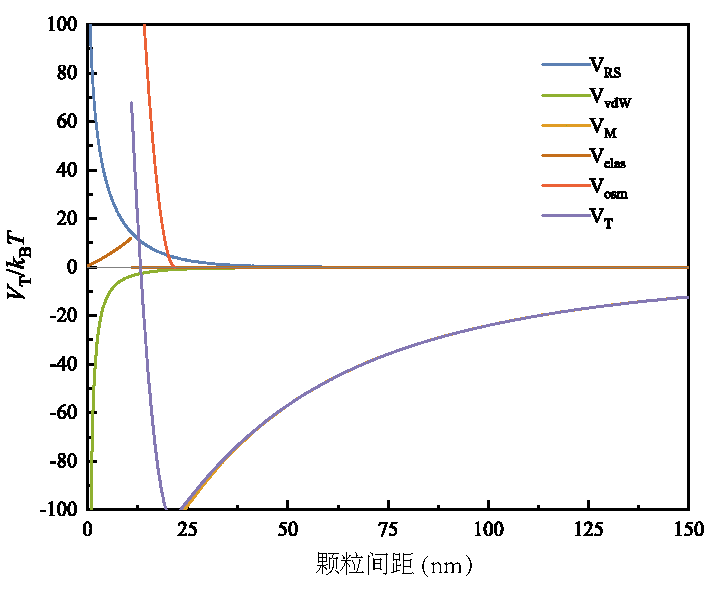
\includegraphics[width=8cm]{figs/fig9.pdf}
        \caption{0.2\%SA-S-NZVI颗粒间相互作用曲线}
        \label{fig9}
	\end{subfigure}

    \begin{subfigure}{8cm}
		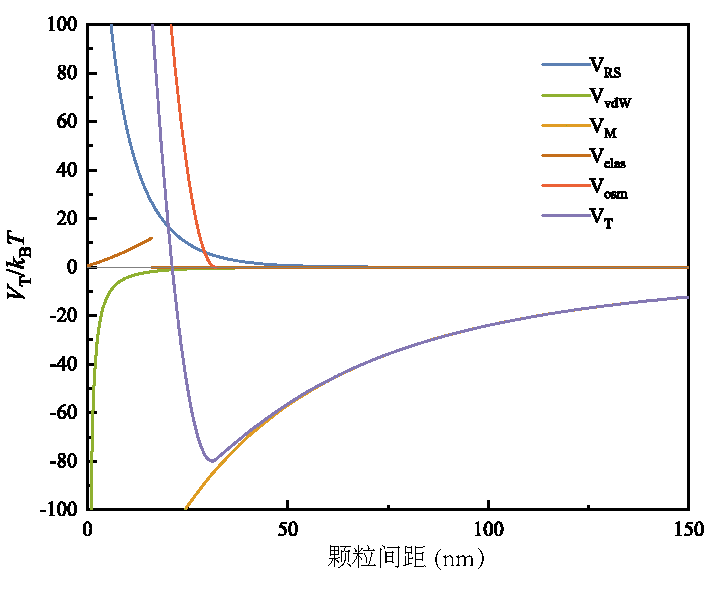
\includegraphics[width=8cm]{figs/fig10.pdf}
        \caption{0.3\%SA-S-NZVI颗粒间相互作用曲线}
        \label{fig10}
	\end{subfigure}
    \bicaption{SA-S-NZVI颗粒间相互作用曲线}{Calculated XDLVO interaction energy for SA-S-NZVI}
\end{figure}

但S-NZVI被海藻酸钠层包覆时,由于表面包覆层的存在,溶液中离子可以穿透SA-S-NZVI粒子表面分散于包覆层内部。假定包覆层是均匀带电的,令$Z$和$N$分别为包覆层中带电基团的价态和密度,则SA-S-NZVI之间的静电势为:\cite{OHSHIMA20152,vskvarla2020unified,2006390}

\begin{equation}
    V_\mathrm{els}(s)=\frac{2 \pi a \rho_\mathrm{fix}^2 \sinh^2(\kappa d)}{\varepsilon _0 \varepsilon _r\kappa ^4}\ln[\frac{1}{1-\exp(-\kappa s)}]
\end{equation}

\begin{equation}
    \rho_\mathrm{fix}=ZeN
\end{equation}

同时,根据Donnan平衡,包覆层中的聚电解质段被吸附固定在颗粒表面,而电离的小离子可以自由移动,因此包覆层附近存在额外渗透压。当颗粒间距不断减小,包覆层逐渐靠近相互重叠增加了局部电解质的浓度,从而提高了局部渗透压($V_\mathrm{osm}$)\cite{2002Electrosteric}。此外,当颗粒之间距离小于$d$时,部分聚合物段被压缩,导致体系的熵减小,从而产生弹性斥力($V_\mathrm{elas}$)\cite{doi:10.1080/07388551.2018.1440525}:

\begin{equation}
    \frac{V_\mathrm{osm}}{k_BT}=\left\{
        \begin{array}{lcl} %lcl左对齐 多行公式
            0& &{2d\leqslant s}\\
            \frac{4 \pi a }{v_1}\cdot\phi _p^2\cdot(\frac{1}{2}-\chi )(d-\frac{s}{2})^2& &{d\leqslant s <2d}\\
            \frac{4 \pi a }{v_1}\cdot\phi _p^2\cdot(\frac{1}{2}-\chi )d^2[\frac{s}{2d}-\frac{1}{4}-\ln(\frac{s}{d})]& &{s<d}
        \end{array}\right.
\end{equation}
\begin{equation}
    \frac{V_\mathrm{elas}}{k_BT}=\left\{
        \begin{array}{lcl}
            0& &{d\leqslant s}\\
            (\frac{2\pi a}{M_w}\cdot\phi_pd^2\rho_p)\{\frac{s}{d}\ln[\frac{s}{d}(\frac{3-s/d}{2})^2]\\ -6\ln(\frac{3-s/d}{2})+3(1+\frac{s}{d}^2)\}& &{d>s}
        \end{array}\right.
\end{equation}

其中,$\chi$为Flory-Huggins常数;$\phi_p$为包覆层聚电解质的体积分数;$d$为包覆层厚度;$v_1$为溶剂分子的体积;$M_w$为聚电解质的分子量;$\rho_p$为聚电解质密度。综上,包覆型S-NZVI的总相互作用能为:

\begin{equation}
   V_\mathrm{T}=V_\mathrm{vdW}+V_\mathrm{els}+V_\mathrm{osm}+V_\mathrm{elas}+V_\mathrm{M} 
\end{equation}

SA-S-NZVI的相互作用势能如\cref{fig8}所示,在短距离上看,体系中主要的排斥力为空间斥力($V_\mathrm{osm},V_\mathrm{elas}$),同时由于包覆层的存在,颗粒的表面电势($V_\mathrm{els}$)要略大于未包覆S-NZVI的静电相互作用($V_\mathrm{el}$),但是仍然无法抵抗S-NZVI自身磁矩的吸引。当SA-S-NZVI相互接近距离小于$2d$时,由于渗透斥力产生极大的能量势垒,阻止SA-S-NZVI的进一步靠近。令$V'_T=0$可求得0.3\%SA-S-NZVI的势能阱分别位于31.10 nm,大小为-79.93 $k_\mathrm{B}T$。综上,0.1 mM电解质溶液中的静电斥力无法抵抗磁力的吸引作用,颗粒主要的斥力来自于空间作用力,因此增加包覆层厚度可以显著减小势能阱的深度。对照未包覆型S-NZVI,不同包覆比的SA-S-NZVI应形成颗粒间距约31 nm的松散团聚体,而非裸S-NZVI的密实团聚体。

\begin{figure}[h]
    \centering
    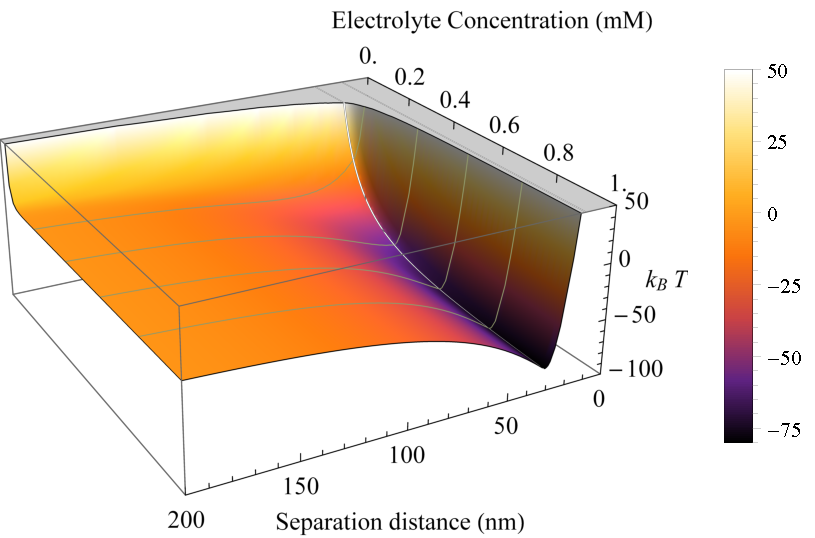
\includegraphics[width=8cm]{figs/fig11.pdf}
    \bicaption{SA-S-NZVI在不同离子强度下的总相互作用能}{Change of DLVO interaction energy for SA-S-NZVI with electrolyte concentration and separation distance}
    \label{fig11}
\end{figure}

由于SA-S-NZVI的附着效率随离子强度增加而提高(\cref{fig4}),颗粒的相互作用受离子强度影响较大。以0.3\%SA-S-NZVI为例,不同离子强度下SA-S-NZVI间的相互作用力如\cref{fig11}所示。低离子强度下颗粒间的静电斥力的大小和作用范围都显著增加,这体现在势能阱由-85.13 $k_\mathrm{B}T$(100.00 mM,图中未画出)快速衰减至-0.07 (0.01 mM)几乎消失。随着电解质浓度提高(>0.5 mM),势能阱深度的变化较小(紫色区域),静电斥力对总势能的影响变得十分有限,颗粒总势能以渗透斥力和磁力主导,最小势能阱维持在-85.13左右,离子强度对其影响可以忽略不计。同时,附着效率的物理意义为颗粒之间发生有效碰撞的几率,因此颗粒聚集的临界混凝浓度由DLVO理论计算可以表示为势能阱的深度大于布朗运动的能量(1.5 $k_\mathrm{B}T$)。要使附着效率达到100\%($\alpha_\mathrm{pp}=1$)则总势能方程需满足:

\begin{equation}
    \left\{
        \begin{array}{lcl} 
            V_T=-1.5\; k_\mathrm{B}T& \\
            V'_T=0 &
        \end{array}\right.
\end{equation}

求得不同包覆比SA-S-NZVI临界浓度分别为$4.53\cdot10^{-2}$ mM,$3.68\cdot10^{-2}$ mM,$4.47 \cdot 10^{-2}$ mM。因此三种包覆比SA-S-NZVI的附着效率在0.1 mM NaCl条件下均为100\%。利用动态光散射法测定$t_0$时刻样品的粒径分布,带入\cref{smoluchowski}计算平均粒径随时间的变化。不同包覆比SA-S-NZVI的平均粒径随时间的变化如\cref{fig2}所示,0.1wt\%、0.2wt\%和0.3wt\%SA-S-NZVI的平均粒径分别增加了133 nm、114 nm、110 nm,可以较好的预测实验结果。

\begin{figure}[h]
    \centering
    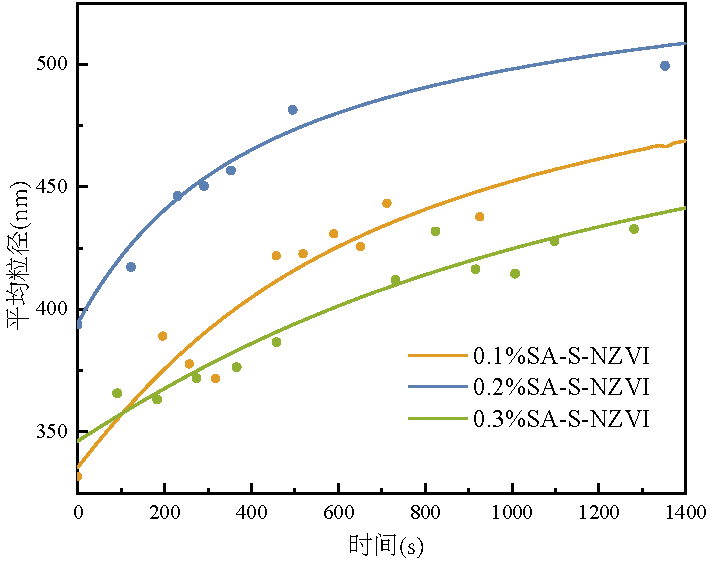
\includegraphics[width=8cm]{figs/fig2.pdf}
    \caption{Changes in mean particle size over time for suspensions of SA-S-NZVI. The curves show the best fit of the aggregation kinetics model to the 0.10 wt\%,0.2 wt\% and 0.3wt\% SA-S-NZVI}\label{fig2}
\end{figure}

为进一步研究SA-S-NZVI的团聚机理,考虑S-NZVI的长程吸引作用主要以磁力为主,而\cref{VM}计算的磁性势能与粒径的6次方正相关,而S-NZVI样品是宽分布的。因此不同粒径颗粒的总势能有显著差异。颗粒粒径,颗粒间距对总势能($V_T$)的变化如\cref{fig12}所示,由于磁性对颗粒粒径敏感,在30\textasciitilde50 nm之间,势能阱的深度随着粒径增加快速滑落,势能阱出现的位置随粒径变化较小。尺寸在30 nm以下的SA-S-NZVI颗粒的势能阱深度仅-0.82 $k_\mathrm{B}T$,小于胶体布朗运动的能量(1.5 $k_\mathrm{B}T$)。因此该条件下SA-S-NZVI形成的聚集不稳定,这可以解释沉降实验中部分SA-S-NZVI保持悬浮的现象。

\begin{figure}[h]
    \centering
    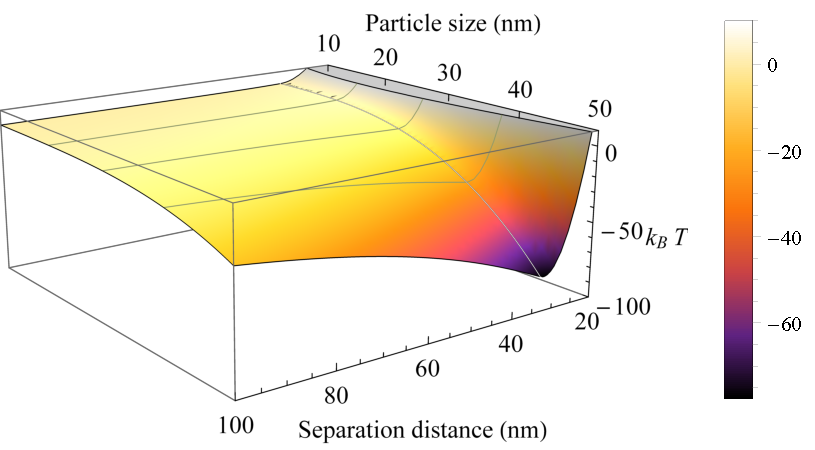
\includegraphics[width=8cm]{figs/fig12.pdf}
    \bicaption{不同离子强度下SA-S-NZVI的XDLVO相互作用}{Change of XDLVO interaction energy for SA-S-NZVI with particle size and separation distance}
    \label{fig12}
\end{figure}

\bisection{本章小结}{Result}

研究了不同的涂层比例和离子强度对裸露和涂层S-NZVI稳定性的影响。结果表明,海藻酸钠的浓度越高,沉降速度越慢。离子强度越高,粘附效率越高,离子强度对不同涂层比例的影响更可以忽略不计。通过软粒子理论计算,不同涂布比例的聚电解质层厚度分别为7.97、10.94和16.62纳米。海藻酸钠的浓度越高,聚电解质层的厚度就越大。用XDLVO理论进一步研究发现,由于S-NZVI的磁效应,颗粒总是倾向于聚结在一起。裸露的S-NZVI没有排斥性的势垒存在,所以会发生不可逆的聚集,应该会形成密集的团聚体。

相比之下,SA-S-NZVI形成31纳米的松散团聚,而不是裸S-NZVI的致密团聚。此外,虽然30纳米以下的小颗粒有结块的倾向,但吸引势能的大小远远小于布朗运动能量,这使得它难以形成稳定的结块。S-NZVI的磁效应随着颗粒间距的增加而缓慢衰减。静电排斥力和空间力的增加只能实现短距离的排斥。然而,它不能避免颗粒在长距离上相互接近的趋势。S-NZVI的磁相互作用随着粒子间距的增加而缓慢衰减。通过削弱S-NZVI的磁性或在系统中加入排斥性的长程力以匹配磁性范围,可以进一步改善S-NZVI的磁性能。

研究了不同包覆比和离子强度对未包覆和包覆型纳米颗粒稳定性的影响。结果表明,海藻酸钠浓度越高,沉降速率越慢。离子强度越大附着效率越高,同时离子强度对不同包覆比的影响较小。采用软粒子理论计算,不同包覆比分别厚度为7.97,10.94,16.62 nm。海藻酸钠浓度越高,包覆层厚度越大。用XDLVO理论进一步研究发现,由于S-NZVI的磁性作用,颗粒始终具有团聚的趋势。裸S-NZVI由于没有斥力势垒存在,发生不可逆团聚,形成密实团聚体。

相比之下,SA-S-NZVI将形成31 nm的松散团聚体,而非裸S-NZVI的致密团聚体,且颗粒尺寸在30 nm以下的小颗粒虽然具有团聚的趋势,但吸引势能远小于布朗运动能量,难以形成稳定的聚集体。而对于30 nm以上的SA-S-NZVI,虽然不可避免发生团聚,但吸引势能小,属于可逆团聚,容易被打散。因此包覆改性大大提升了S-NZVI在水中的分散能力。此外,由于S-NZVI的磁力作用随着颗粒间距增加衰减缓慢,增加静电斥力和空间作用力仅能实现短距离的排斥而无法避免颗粒长距离上相互靠近的趋势。由此可见,要实现NZVI在水溶液中真正的稳定,在后续研究中可以通过削弱S-NZVI的磁性,或在体系中增加与磁性作用范围相匹配的长程斥力以进一步提高S-NZVI的分散效果。
\bichapter{改性硫化型纳米零价铁的稳定性研究}{Study on stabilization
of coated sulfur-modified NZVI}


\bisection{pH对不同包覆比的S-NZVI稳定性的影响}{Effect of pH on the stability of S-NZVI with different coating ratios}

如\cref{fig3}所示,未包覆的S-NZVI在酸性条件下时$\zeta$电位为正,碱性条件下为负,等电点在pH=7.0附近,此时颗粒表面静电力变小,排斥力减弱。由于通常地下水的pH范围在6.5到8.5之间\cite{dixiashuibiaozhun},因此该环境下未包覆的S-NZVI胶体团聚速率快,更易脱稳沉降,与相关研究结果相符。为模拟地下水环境,调节pH=8,因此本研究中的硫化纳米铁表面带负电。

\begin{figure}[h]
    \centering
    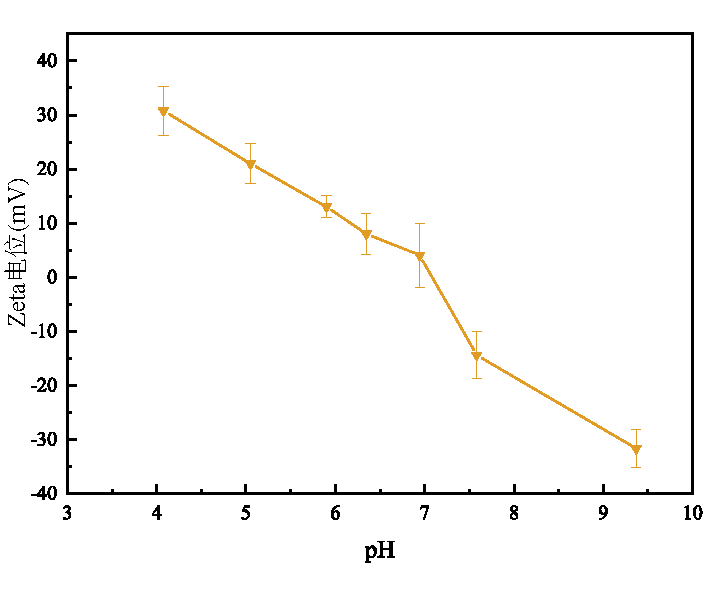
\includegraphics[width=12cm]{figs/fig3.pdf}
    \caption{不同pH裸S-NZVI的$\zeta$电位}{Zeta potential of bare S-NZVI as a function of pH}\label{fig3}
\end{figure}

\bisection{不同包覆比下S-NZVI的稳定性}{Stability of S-NZVI at different coating ratios}

纳米颗粒在水中同时受到扩散和重力沉降作用,如果纳米粒子的扩散克服了沉降作用,那么纳米粒子可以保持很长时间的稳定。其中重力作用与粒子半径的平方成正比,扩散作用与粒子尺寸成反比,当纳米粒子聚集成微米大小的团簇时,由于扩散作用小于沉降作用,团聚体会沉降到容器的底部。所以沉降速率是表征S-NZVI胶体稳定性的良好指标。

\begin{figure}[h]
    \centering
    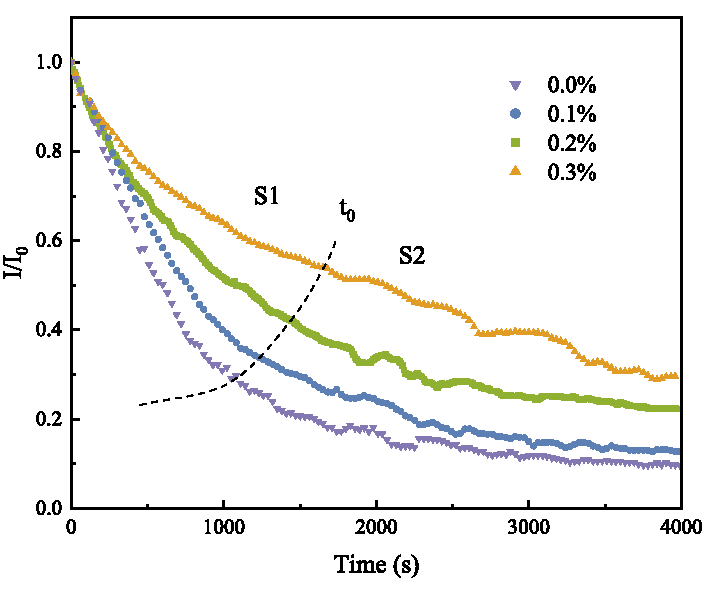
\includegraphics[width=12cm]{figs/fig1.pdf}
    \caption{不同包覆比和裸S-NZVI的沉降曲线}{Sedimentation curves of bare and modified S-NZVI}\label{fig01}
\end{figure}

如\cref{fig01}所示,未包覆的S-NZVI的沉降可分为两个阶段:在S1阶段,样品中存在大量超过临界尺寸的颗粒,因此快速沉降。在$t_0$时刻,多数大颗粒沉降完成,沉降速率降低,样品进入S2缓慢沉降阶段,逐渐趋于稳定。

海藻酸钠包覆S-NZVI的沉降模式与未包覆材料相同,均由S1、S2两个阶段组成,但由于聚电解质层的存在,包覆硫化钠米铁的沉降速率与海藻酸钠浓度负相关。海藻酸钠浓度越大,S1阶段的沉降速率越小,S2阶段保持悬浮的颗粒数量越多,体系的稳定性越好。

\bisection{离子强度对SA-S-NZVI稳定性的影响}{Effect of ionic strength on the stability of SA-S-NZVI}

金属氧化物纳米颗粒在水溶液中的稳定性在很大程度上取决于离子强度。为了研究离子强度对SA-S-NZVI在溶液中的稳定性(pH=$8\pm 0.1$),制备不同包覆比(0、0.1、0.2、0.3wt\%)的SA-S-NZVI,采用NaCl调节离子强度(0.00$\sim$100 mM NaCl)。颗粒之间的附着效率由\cref{alpha_ppexp}计算,其中$k_{\mathrm{fast}}$取扩散限制团聚阶段下$k$的平均值。

\begin{figure}[h]
    \centering
   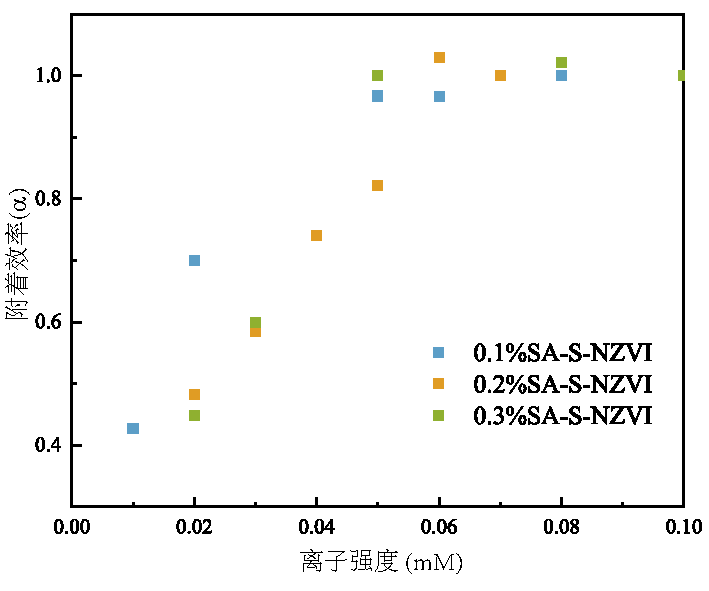
\includegraphics[width=12cm]{figs/Graph1.png}
    \bicaption{不同离子强度下包覆型S-NZVI的附着效率}{Influence of iron strength on aggreation behaviors of modified S-NZVI}\label{fig4}
\end{figure}

实验结果如\cref{fig4}所示,不同包覆比的SA-S-NZVI与裸S-NZVI随着离子强度的增加,在低浓度NaCl下,NaCl浓度的增加将提高电荷屏蔽的程度,从而提高团聚速率,这反映在附着效率的提高上。该过程中,附着效率与NaCl的投加量正相关,这种团聚过程称为反应限制团聚$(\alpha<1)$。在高NaCl浓度下,SA-NZVI的电荷被完全屏蔽,势垒消失,该过程中颗粒发生扩散限制团聚$(\alpha=1)$,团聚速率达到最大值,且与NaCl投加量无关。NaCl对不同包覆比S-NZVI的临界浓度均在0.05\textasciitilde0.06 mM附近。

\bisection{聚电解质包覆层的特性}{Characteristics of the polyelectrolyte
layers}

颗粒间空间斥力的大小和作用范围与表面吸附的聚合物浓度和包覆层厚度有关。不同包覆比的S-NZVI的电泳迁移率随离子强度的变化如\cref{fig5}所示,其中曲线由测量的平均电泳迁移率\cref{psidon,psi0,ue}拟合得到,各参数见\cref{tb1}。

由于包覆层的存在,SA-S-NZVI周围的扩散层被压缩,其电泳迁移率随离子强度的变化较未包覆S-NZVI小。随着离子强度不断提高,未包覆S-NZVI的电泳迁移率逐渐趋于零,而不同包覆比的SA-S-NZVI(0.1\%wt,0.2\%wt,0.3\%wt)受包覆层特性影响分别趋于-2.8,-2.2和-2.3 $\mathrm{\mu m\, s^{-1}\, cm\,V^{-1}} $。

由于软粒子对滑移面位置不敏感\cite{1992Electrophoretic},Smoluchoski公式以硬粒子为基础并不适用于包覆型S-NZVI。根据Ohshima的软粒子理论计算的包覆型S-NZVI的表面电荷$\psi_0$远小于由Smoluchoski公式计算的$\zeta$电位。因此,软粒子并不适用于传统DLVO理论的双电层公式计算静电斥力。

\begin{figure}[h]
    \centering
    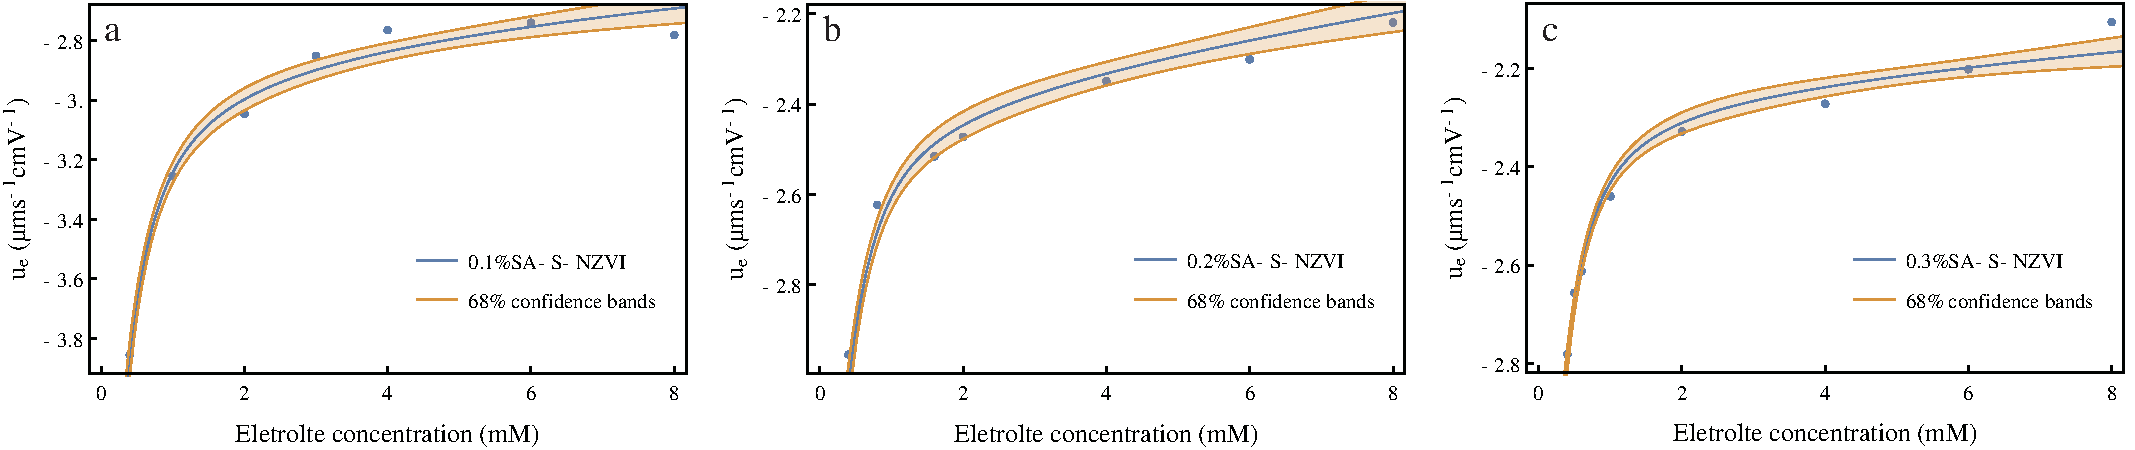
\includegraphics[width=12cm]{figs/fig5.pdf}
    \bicaption{不同NaCl浓度下包覆型S-NZVI的电泳迁移率}{Electiophoretic mobility of the sodium alginate coated S-NZVI as a function of NaCl (mM)}
    \label{fig5}
\end{figure}

\begin{table}
    \centering
    \bicaption{利用Ohshima软粒子理论计算pH值为8.0$\pm $0.1时吸附聚电解质层的特性  }{Characteristics of the adsorbed polyelectrolyte layers at pH 8.0$\pm $0.1 as estimated by Ohshima’s soft particle analysis}\label{tb1}
    \begin{tabular}{@{}ccccc@{}}
        \toprule
         样品类型 & $ZN$/$\mathrm{N_A}$& $d$ & $1/\lambda$ &$\phi_p$\\
           &$(\mathrm{mol/m^3})$&(nm)&(nm)& $(10^{-3})$ \\
        \midrule
        0.1\%SA & 3.28$\pm$1.08 & 7.97$\pm$4.11 & 6.63$\pm$0.58 & 113\\
        0.2\%SA & 1.47$\pm$1.25 & 10.94$\pm$4.68 & 8.51$\pm$1.06 & 80\\
        0.3\%SA & 1.50$\pm$1.39 & 16.62$\pm$4.58 & 9.57$\pm$1.97 & 54\\
        \bottomrule
    \end{tabular}
\end{table}


包覆层中聚电解质的体积分数是影响颗粒稳定性的重要因素。根据计算的颗粒平均包覆层厚度和吸附浓度估算吸附到NZVI表面聚电解质的体积分数:

\begin{align}
    \phi_p=& \frac{\Gamma\cdot 4\pi a^2}{\rho_p\cdot \frac{4}{3}\pi [(d+a)^3-a^3]}  \\
    =&\frac{3\cdot\Gamma a^2}{\rho_p[(d+a)^3-a^3]} \nonumber
\end{align}

其中,$\rho_p$是聚电解质密度;$d$为包覆层厚度;$a$为颗粒粒径;$\Gamma$为S-NZVI表面聚电解质的吸附浓度,制备样品吸附后通过差量法利用总有机碳分析仪测量TOC计算。

\bisection{本章小结}{Result}

% bibliography, glossary and index would go here.
\begin{conclusion}

还

\section*{结论}

没

\section*{展望}

编

\end{conclusion}
\makebib{ref/reference}

\appendix
% \biappendix{两情若是久长时}{Liangqingruoshijiuchangshi}
\zhlipsum[1-3][name=simp]

% \biappendix{又岂在朝朝暮暮}{You qi zai zhao zhao mu mu}

\zhlipsum[11-12][name=simp]

\backmatter
\begin{publication}
	内容...
\end{publication}
\bichapter*{致谢}{Acknowledgement}

\end{sloppypar}
\end{document}